\section{Umsetzung}
\textcolor{red}{Zum Schluss der Arbeit kann in dem letzten Teil eine thesenartige Zusammenfassung der Untersuchungsergebnisse gegeben werden. Andere Möglichkeiten sind hier auch der Ausblick auf weitere – noch ungelöste – Fragestellungen im Zusammenhang mit dem Thema.}

\subsection{Einrichtung der Datenbank}

\begin{figure}[ht!]
  \centering
  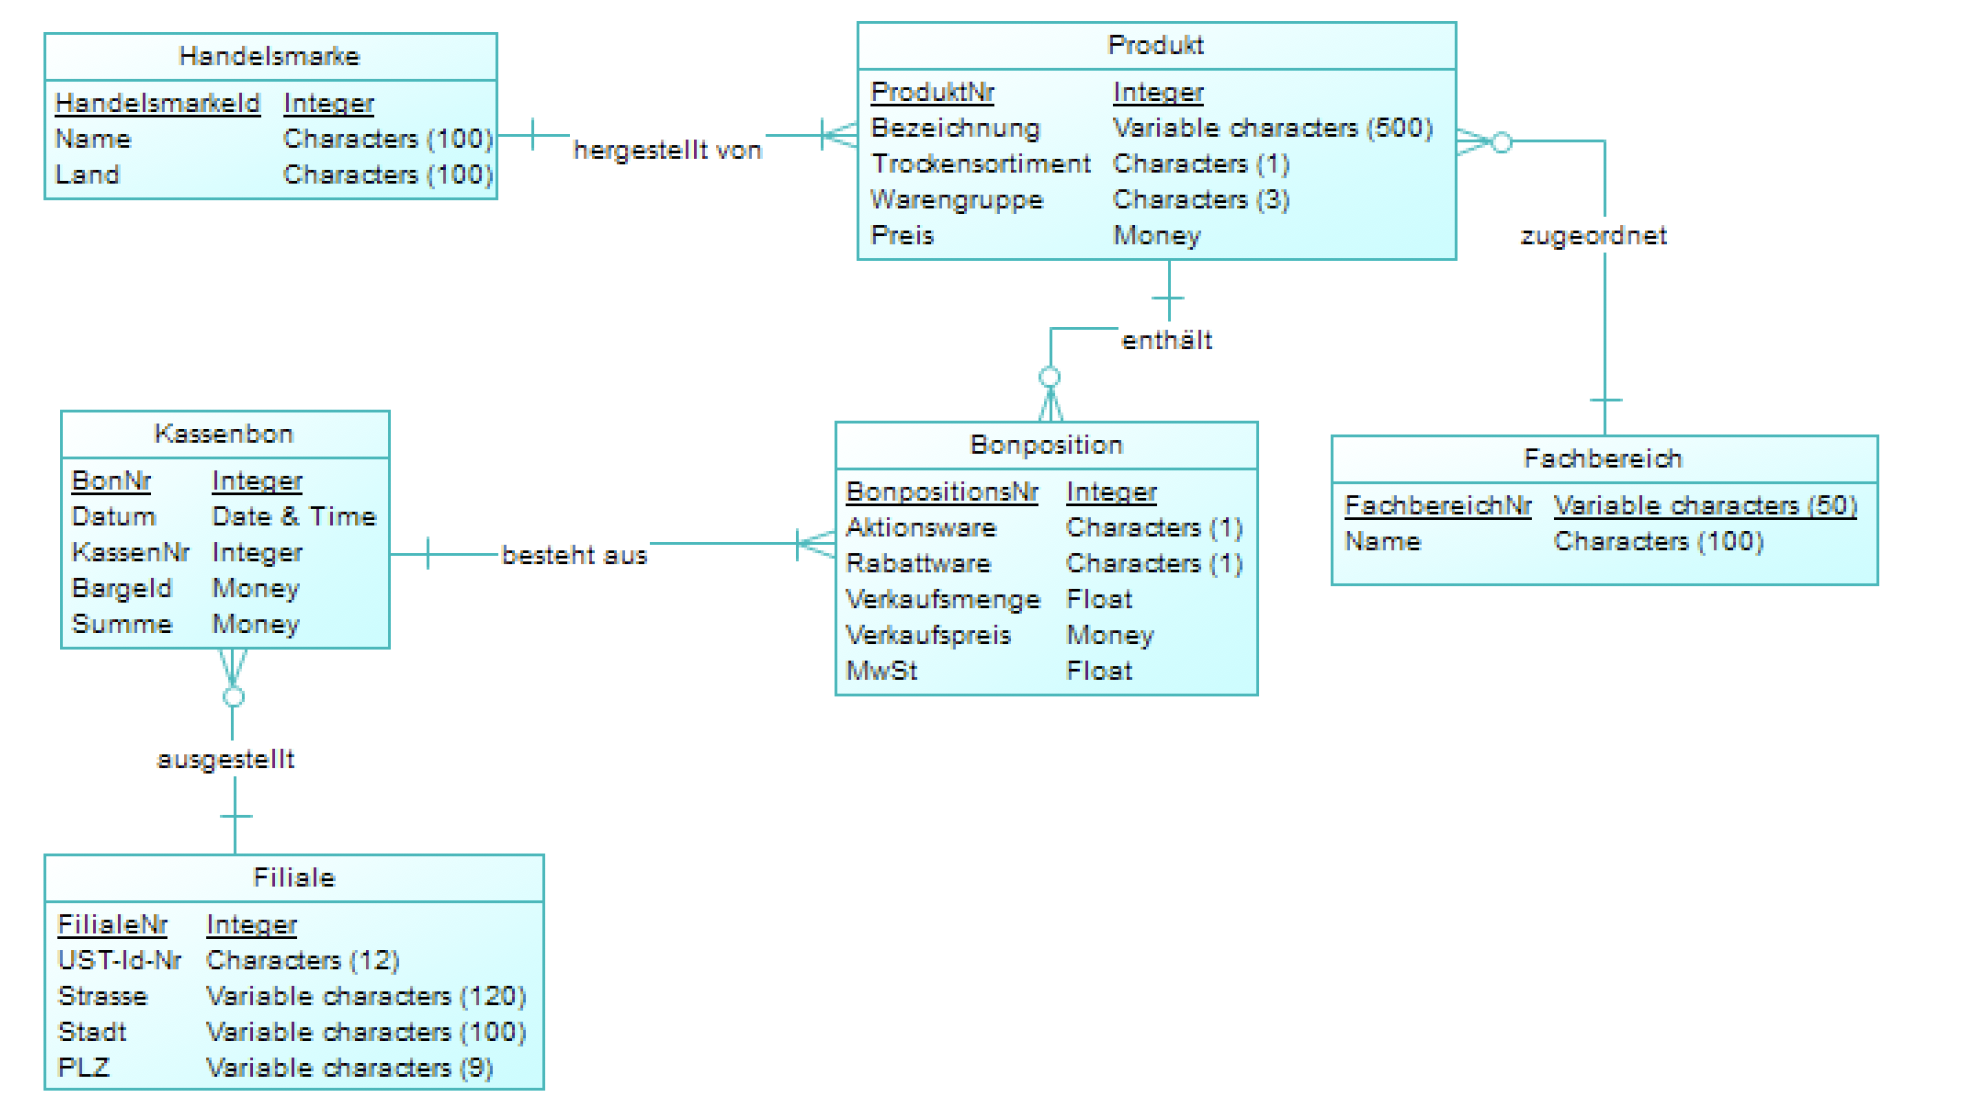
\includegraphics[width=1.2\linewidth]{pictures/db_basic.png}
  \caption[ER-Modell zur Auswertung von Kassenbons]{ER-Modell zur Auswertung von Kassenbons (Quelle: DBIS-Aufgaben)}
\end{figure}

\subsection{Java-Programm}


\begin{figure}[ht!]
  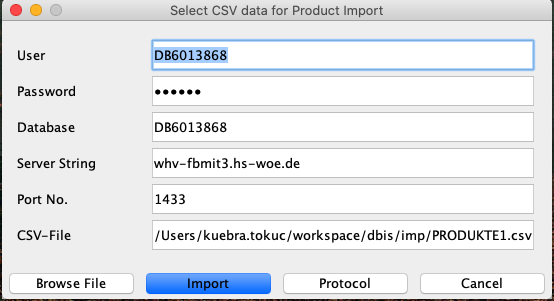
\includegraphics[width=1\linewidth]{window.png}
  \caption{Importfenster des Java-Programms}
\end{figure}


\textcolor{red}{\blindtext}

\subsection{Data Warehouse}

\subsubsection{Erweiterung des Datenbestandes}

\subsubsection{Aufbereitung des Datenbestandes}

\subsubsection{Analyse des Starschemas}

Nachdem der Datenbestand erweitert und korrekt aufbereitet worden ist, wird ein Starm-Schema für ein Data-Warehouse zur Umsatzanalyse und Auswertung von Verkaufsdaten nach einem vorliegenden Schema (s. Abbildung \ref{dw_concept}) erstellt. Das Star-Schema besteht aus Dimensionen- und Faktentabellen, welche die Struktur und den Inhalt einer multidimensionalen Datenmenge definieren \citep{Wulff2019}. Die Werte in der Faktentabelle werden durch die Primary Keys der Dimensionstabelle mit ihr in Abhängigkeit gebracht (s. Abbildung \ref{dw_phys}). Allerdings ergibt die Analyse des Datenmodells Inkosistenzen zwischen den verschiedenen Tabellen:

\begin{enumerate}
  \item Kein Fachbereich im Sternschema, stattdesen Abteilung
  \item Kassenbon\_Fakten AbteilungsNr FK int und DIM\_Abteilung AbteilungsNr PK int
  \item FilialeNr int der operativen DB und FilialeNr char(3) der DIM\_Filiale
  \item Warengruppe char(3) der operativen DB (ODB) und Warengruppe char(1) der DIM\_Produkt
  \item Bezeichnung des Produkts in ODB varchar(500) und in DIM\_Produkt varchar(100)
\end{enumerate}


\begin{figure}[ht!]
  \centering
  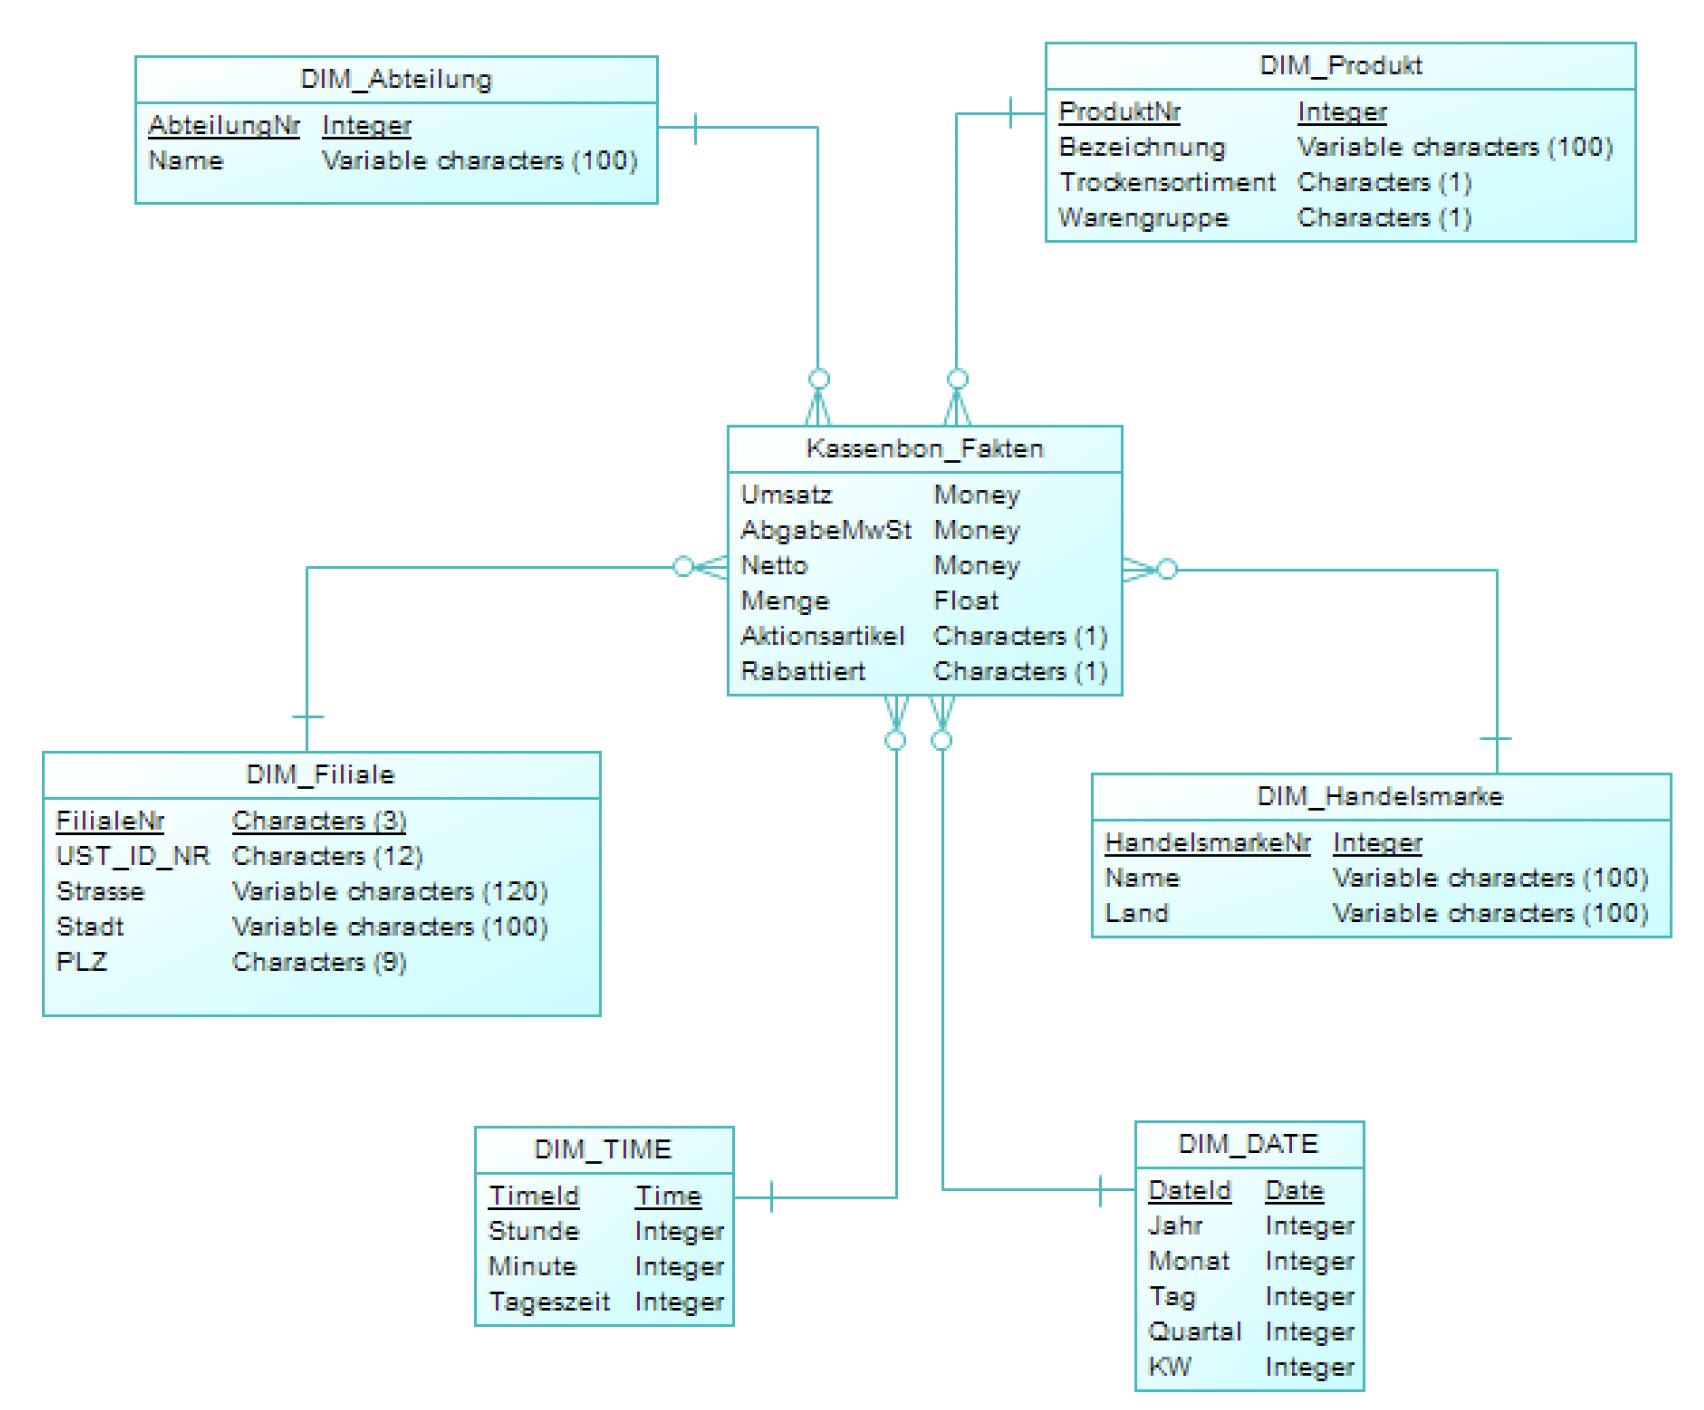
\includegraphics[width=1.1\linewidth]{pictures/dw_concept.png}
  \caption[Konzeptionelles Datenmodell des Data-Warehouses]{Konzeptionelles Datenmodell des Data-Warehouses (Quelle: DBIS-Aufgaben)}
  \label{dw_concept}
\end{figure}

\begin{figure}[ht!]
  \centering
  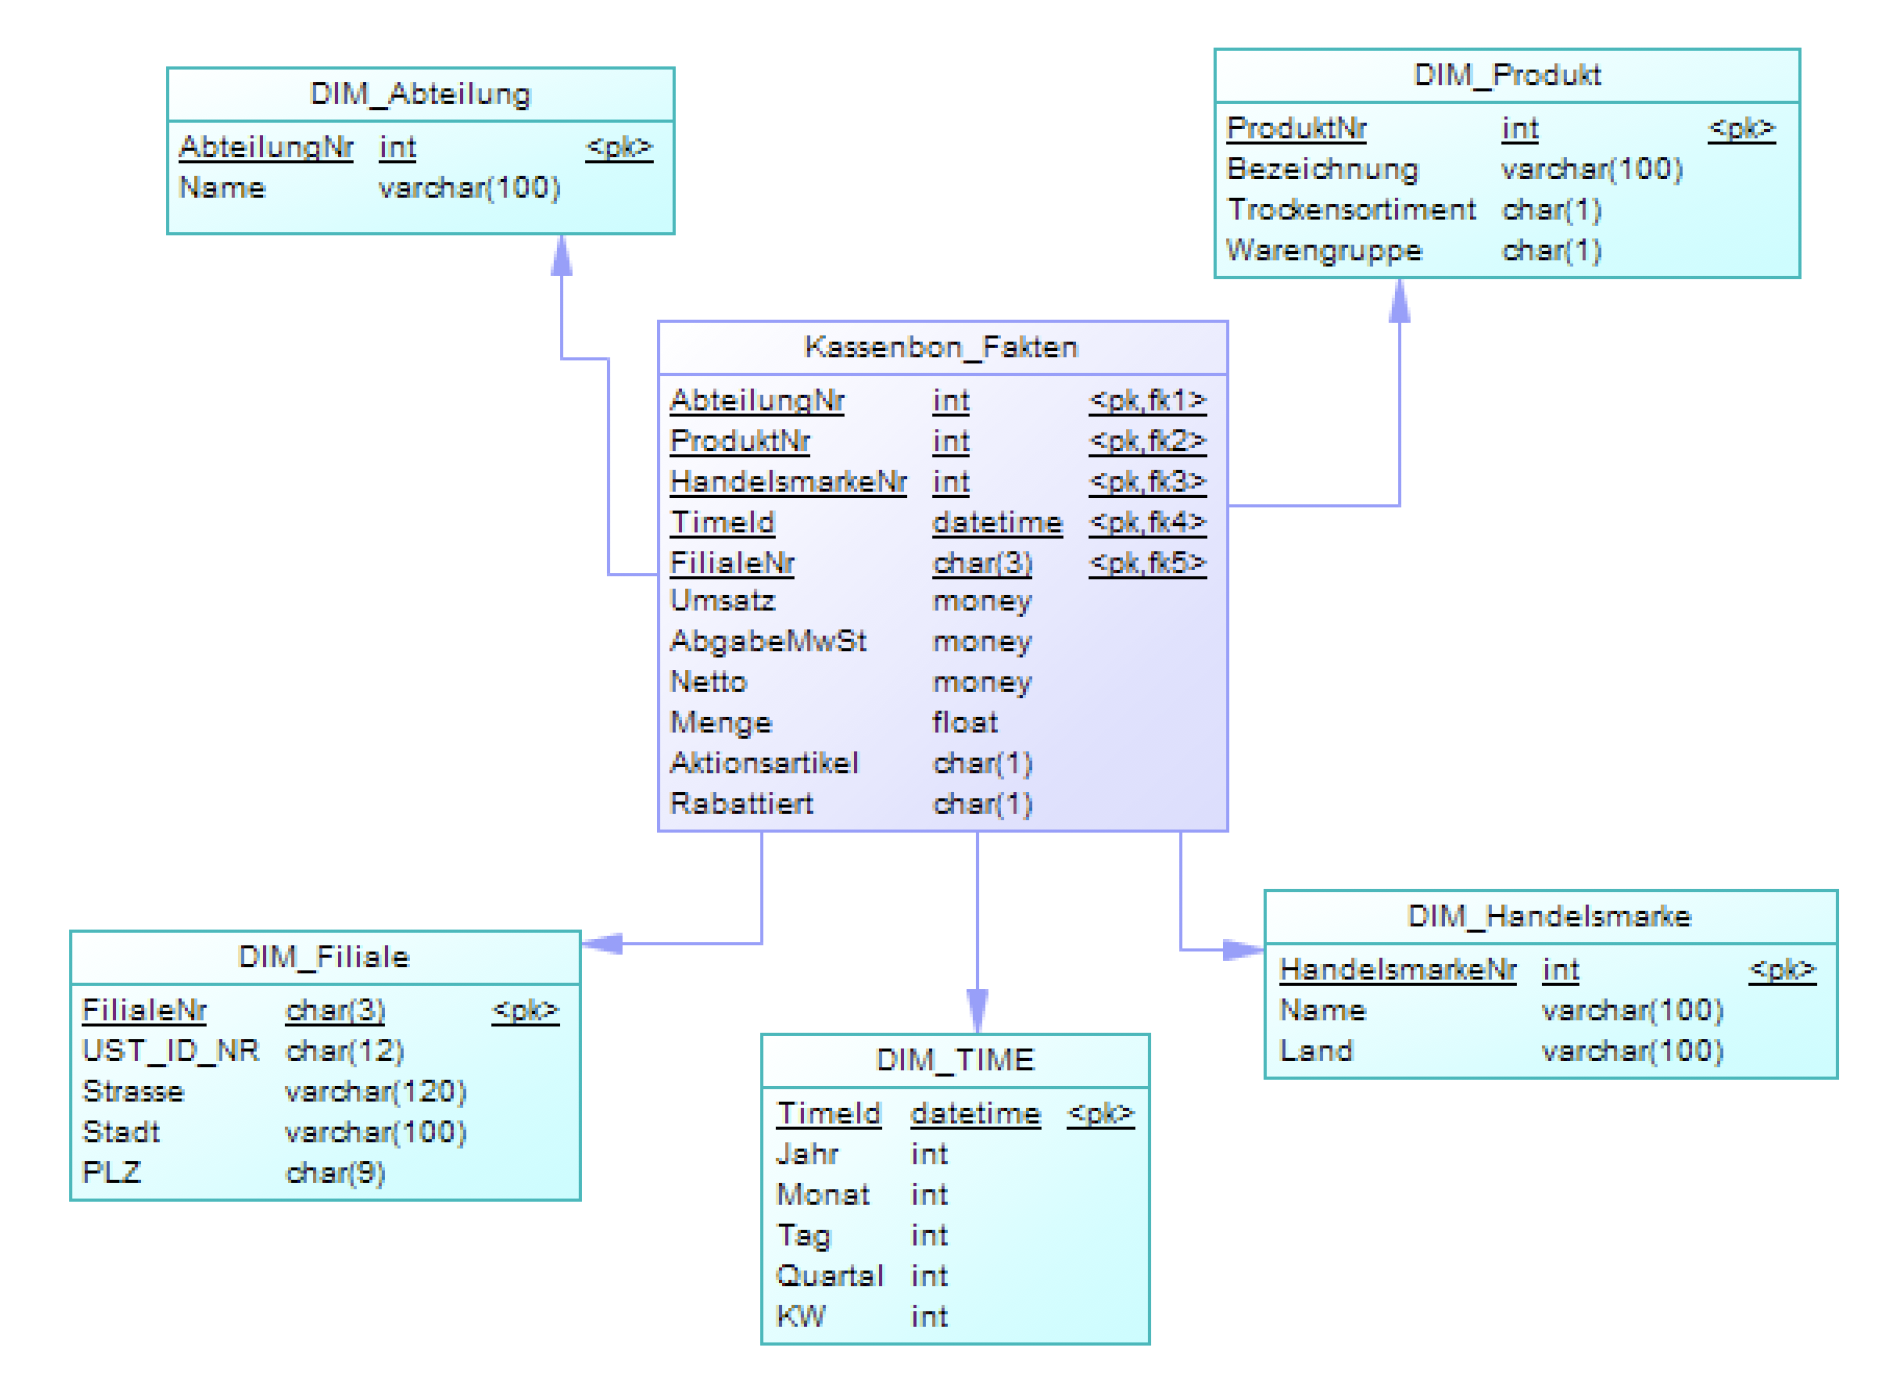
\includegraphics[width=1.1\linewidth]{pictures/DW_Physical_Data.png}
  \caption[Physikaliches Datenmodell des Data-Warehouses]{Physikaliches Datenmodell des Data-Warehouses (Quelle: DBIS-Aufgaben)}
  \label{dw_phys}
\end{figure}

\begin{figure}[ht!]
  \centering
  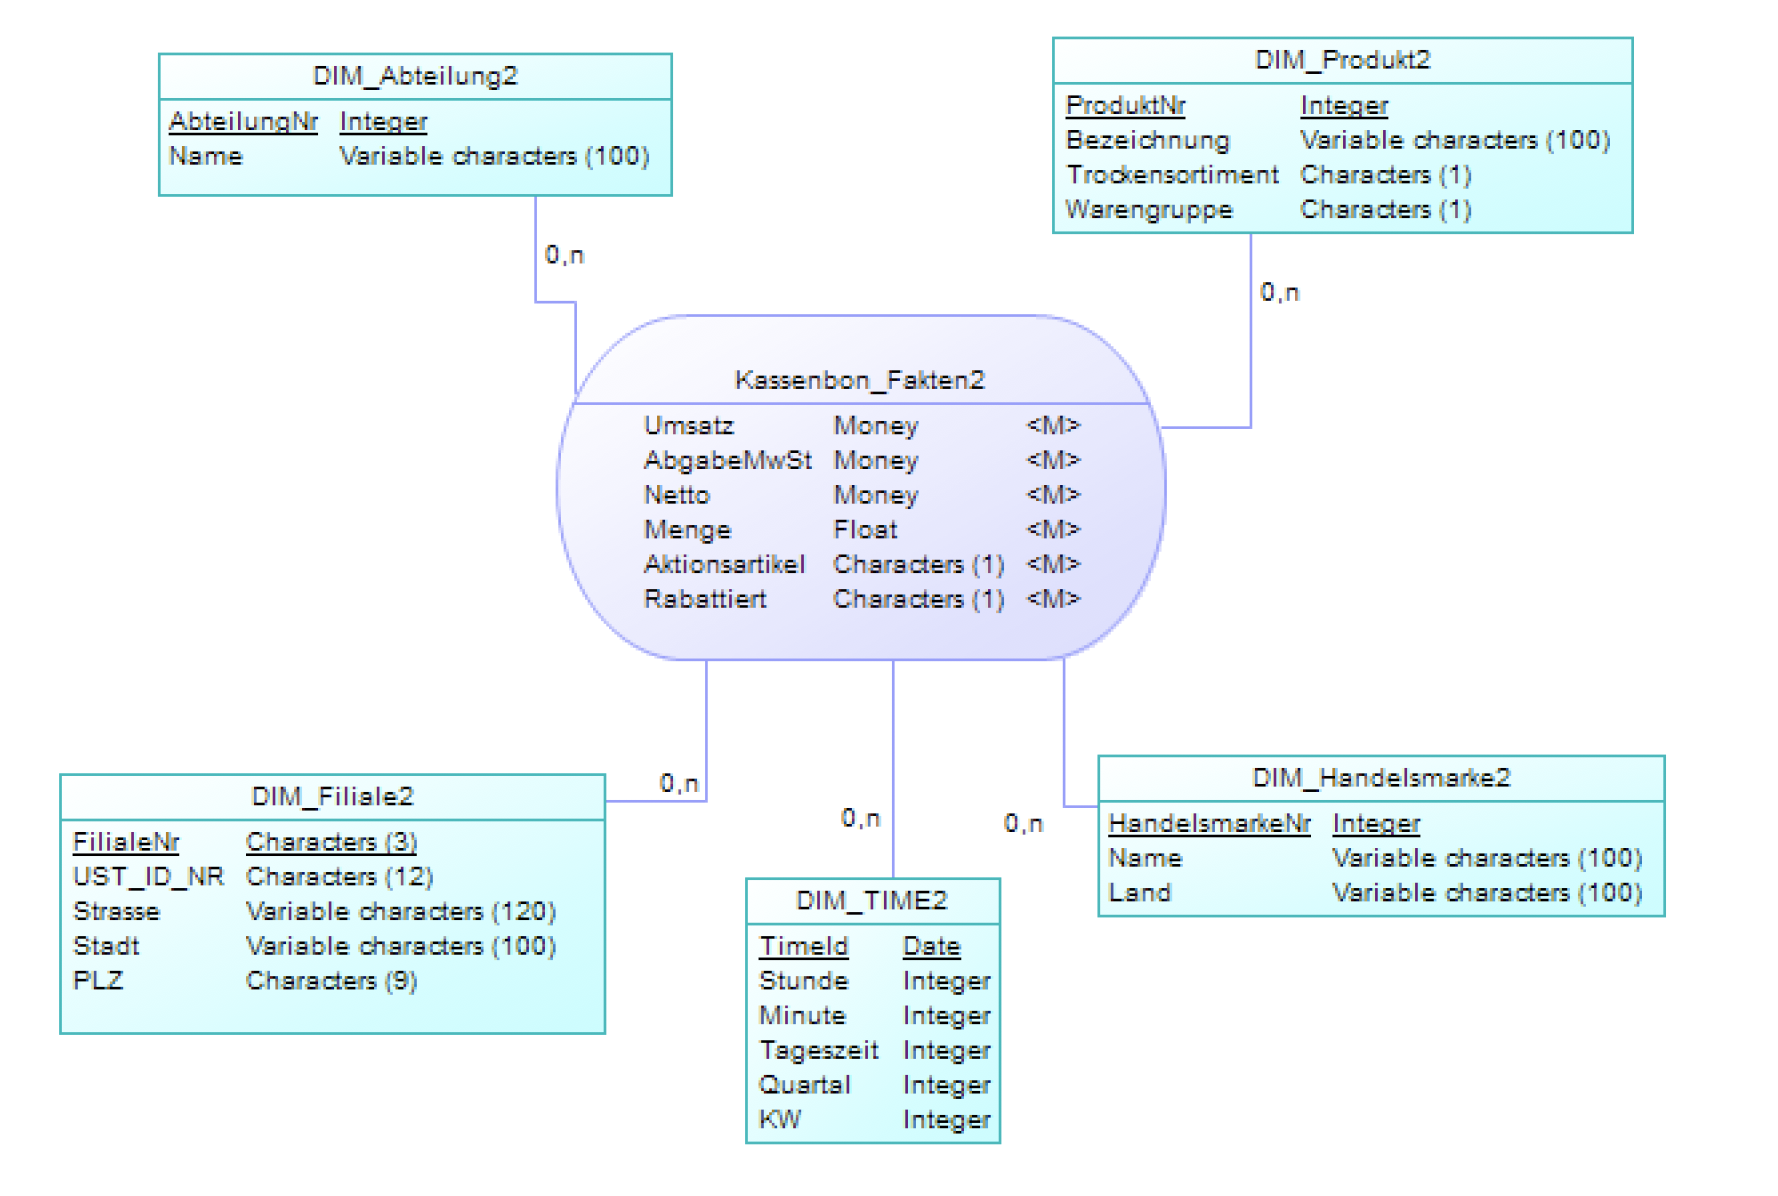
\includegraphics[width=1.1\linewidth]{pictures/dw_asso.png}
  \caption[Datenmodell des DW mit Assoziierung]{Datenmodell des DW mit Assoziierung (Quelle: DBIS-Aufgaben)}
  \label{dw_asso}
\end{figure}

\subsubsection{ETL-Prozess}

Mit dem ETL-Prozess (Extract, Transform, Load) werden die Daten aus der operativen Datenbank für die Auswertung und Analyse für das Laden in das Data-Warehouse aufbereitet.


\subsubsection{Aggregate auf Wochenbasis}

\begin{figure}[ht!]
  \centering
  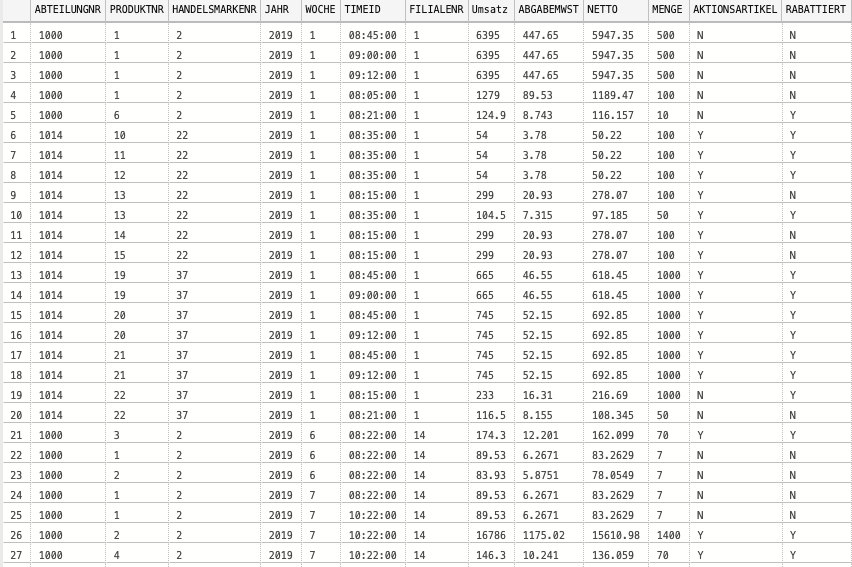
\includegraphics[width=1.1\linewidth]{pictures/fakten_woche.png}
  \caption{Aggregate auf Wochenbasis}
  \label{fakten_woche}
\end{figure}


\textcolor{red}{\blindtext}

\subsection{Prozedur für das Reporting}

\begin{figure}[ht!]
  \centering
  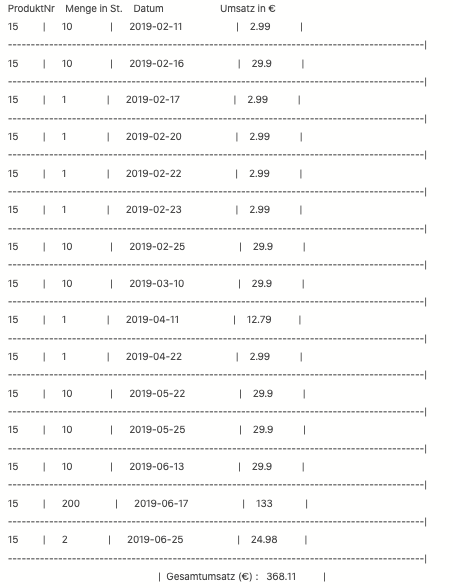
\includegraphics[width=1.1\linewidth]{pictures/report_sql.png}
  \caption{Reporting-Tabelle}
  \label{report_sql}
\end{figure}

\subsection{Reporting mit QlikSense}

\textcolor{red}{\blindtext}

\newpage

